\newpage
\restoregeometry
\section{Grundlagen}
\subsection{Radarfernerkundung}
Bei der Radarfernerkundung werden vom Radarsystem in regelmäßigen Abständen elektromagnetische Signale ausgesandt. Nach dem Senden eines Signals 
(Chrip) folgt ein Zeitfenster indem die Plattform auf Echos des ausgesandten Signals wartet.
Trifft das ausgesandte Signal auf eine Oberfläche, zum Beispiel 
die Erdoberfläche, wird ein Bruchteil reflektiert und als Echo vom Fernerkundungssystem empfangen \cite{tutorial_on_sar}.

Die Radarfernerkundung gehört zu den aktiven Fernerkundungsmethoden da hier im Gegensatz zur optischen Fernerkundung nicht nur 
von Oberflächen reflektierte Strahlung von anderen Strahlungsquellen wie der Sonne aufgenommen wird, sondern das Fernerkundungssystem 
selbst als Strahlungsquelle dient. Messungen können daher tageszeitunabhängig erfolgen. Dabei können die sendenden und erfangenden Komponenten 
unterschiedlich (bi- oder multistatisches Radar) oder identisch sein (monostatitsches Radar). Bildgebende Radarsysteme werden auf mobilen Plattformen 
montiert und blicken seitlich auf die zu beobachtende Oberfläche. Die Flugrichtung wird Azimut und die Blickrichtung als Slant Range 
bezeichnet \cite{tutorial_on_sar} (Abbildung 1). 

Die Eigenschaften des reflektierten Signals hängen sowohl von Parametern des Aufnahmesystems als von Parametern der reflektierenden Oberfläche ab.
So werden in der Radarfernerkundung verschiedenen Frequenzbänder verwendet, welche sich in Frequenz und Wellenlänge unterscheiden. Da sich Wechselwirkung zischen Signalen 
unterschiedlicher Frequenzbänder unterscheidet können so unterschiedliche Aspekte der beobachteten Oberfläche hervorgehoben werden. Dabei kommen in der Regel
Wellenlängen von 0.75m bis 120m zu Einsatz (Tabelle 1).
Mit einer größeren Wellenlänge kann ein Medium auch tiefer durchdrungen werden. Außerdem werden Wolken, Dunst und Rauch durchdrungen was den zusätzlich Vorteil bietet
wetterunabhängig Messungen durchführen zu können \cite{einfuehrung_in_fernerkundung}.

\begin{table}[H]
    \caption{Gängige Frequenz-Bänder in der Radarfernerkundung \cite{tutorial_on_sar}}
    \centering
    \begin{tabular}{|c|c|c|c|c|c|c|c|} 
        Frequenzband & Ka & Ku & X & C & S & L & P\\ 
        \hline
        Frequenz (GHz) & 40-25 & 17.6-12 & 12-7.5 & 7.5-3.75 & 3.75-2 & 2-1 & 0.5-0.25\\ 
        Wellenlänge (cm) & 0.75–1.2 & 1.7–2.5 & 2.5–4 & 4–8 & 8–15 & 15–30 & 60–120\\ 
    \end{tabular}
    \label{table:1}
\end{table}

Die Durchdringungstiefe hängt auch von der Dielektrizitätskonstante der reflektierenden Oberfläche ab. Ist diese groß, reflektiert die Oberfläche stark und die 
Durchdringungstiefe ist gering. Die Rauigkeit ist eine Eigenschaft der reflektierenden Oberfläche und hat großen Einfluss auf das reflektierte Signal. Ist diese im Verhältnis
zur verwandten Wellenlänge gering so kommt es zur Spiegelung und nur ein geringer bis kein Anteil des kehrt zum Empfänger zurück. Doch auch die Form und Exposition der Oberfläche 
nimmt Einfluss auf das reflektierte Signal. So werden Flächen unterschiedlich stark bestrahlt. Ist eine dem System abgewandte Fläche steiler geneigt als der Depressionswinkel 
liegen Sie sogar im Radarschatten und werden gar nicht bestrahlt \cite{einfuehrung_in_fernerkundung}. 
Zusätzlich ist die Polarisation der ausgesandten und empfangenen Signale bei der Messung ausschlaggebend. Sie können horizontal oder 
vertikal polarisiert sein. Dies führt zu vier möglichen Polarisationsmodi für das Senden (transcieve) und das Empfangen (receive) nämlich HH, VV, HV und VH. Auch die 
Polarisation sorgt für eine unterschiedliche Wiedergabe von beobachteten Objekten und kann somit verwendet werden um bestimmte Aspekte hervorzuheben
 \cite{einfuehrung_in_fernerkundung}. Die Auflösung entlang des Azimut unterscheidet sich von der Auflösung in Blickrichtung. Die Auflösung in Azimutrichtung wird von 
 der Antennenlänge bestimmt da diese festlegt wie lange die Reflektion eines Objektes empfangen werden. Die Antennenlänge kann bauartbedingt nicht beliebig gesteigert werden.
Die Antennenlänge bestimmt auch den Abstrahlwinkel und somit die Ausdehnung am Boden eines Impulses in Azimutrichtung. Diese nimmt mit zunehmender Entfernung
zu, während die Auflösung abnimmt.
Die Auflösung in Blickrichtung hängt vom Depressionswinkel der Antenne ab da dieser Einfluss auf die Laufzeit des Signals nimmt. Die Ausdehnung des beobachteten Gebietes 
hängt von der Laufzeit des ausgesandten Signales ab. Die Objekte werden abhängig von ihrer Entfernung zur Antenne verzerrt wiedergegeben da nahegelegende Objekte von der
Wellenfront schneller durchlaufen werden. Dieser unterschied zwischen Schrägdistanz und Bodendistanz lässt sich jedoch nahezu vollständig korrigieren 
\cite{einfuehrung_in_fernerkundung}. Die bisher beschriebene System wird auch System mit realer Apertur bezeichnet und eignet sich nur für geringe Flughöhen da hier 
der Abstand zwischen Antenne und Oberfläche gering ist. Bei Radarsystemen mit einer synthetischen Apertur wird durch die Bewegung des Sensors in Azimutrichtung die 
wirksame Antennenlänge rechnerisch verlängert indem die reflektierten Signale eines beobachteten Objektes von verschiedenen Standpunkten und unterschiedlichen Zeitpunkten 
miteinander korreliert werden. So können hohe Azimutauflösungen erzielt werden. Solche Systeme eigenen sich auch für den Einsatz auf Satelliten \cite{einfuehrung_in_fernerkundung}. 

\begin{figure}[H]
    \centering
    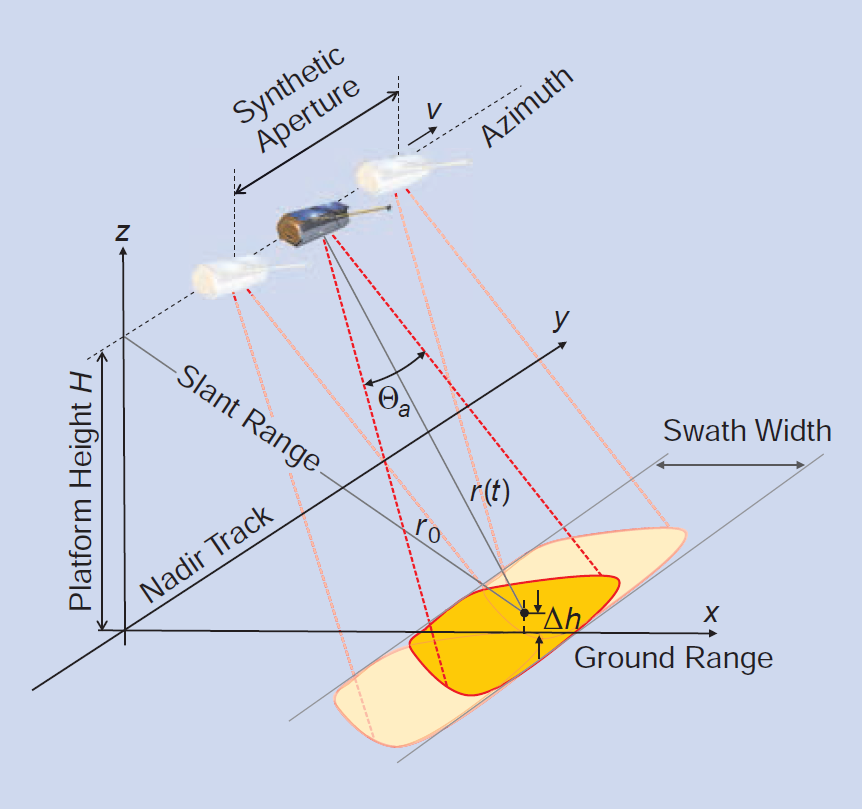
\includegraphics[width=0.5\textwidth]{Bilder/SAR_Prinzip.png}
    \caption{Prinzip eines SAR Fernerkundungssystems \cite{tutorial_on_sar}}
    \label{fig:sar_prinzip}
\end{figure}

Solche Systeme können in unterschiedlichen Aufnahmeverfahren arbeiten. Das einfachste dieser Verfahren ist das Strip-Map Verfahren bei dem nur ein Streifen 
kontinuierlich aufgenommen wird. Breitere Aufnahmestreifen können mit dem ScanSAR Verfahren erzielt werden. Dabei werden unter verschiedenen Depressionswinkeln, 
in Blickrichtung und zeitversetzt mehrere Sub-Aufnahmestreifen erzeugt. Im Vergleich zum Strip-Map Verfahren ist Auflösung jedoch geringer. 
Wird eine höhere Auflösung benötigt kann das Spotlight Verfahren zum Einsatz kommen bei dem eine fixe Region über einen längeren Zeitraum hinweg beobachtet wird. Dies führt zu 
einer sehr langen wirksamen Antenne und damit zu hohen Azimutauflösungen. 
Angepasste Verfahren oder Mischformen können je Beobachtungsszenario zum Einsatz kommen \cite{tutorial_on_sar}. 

\begin{figure}[H]
    \centering
    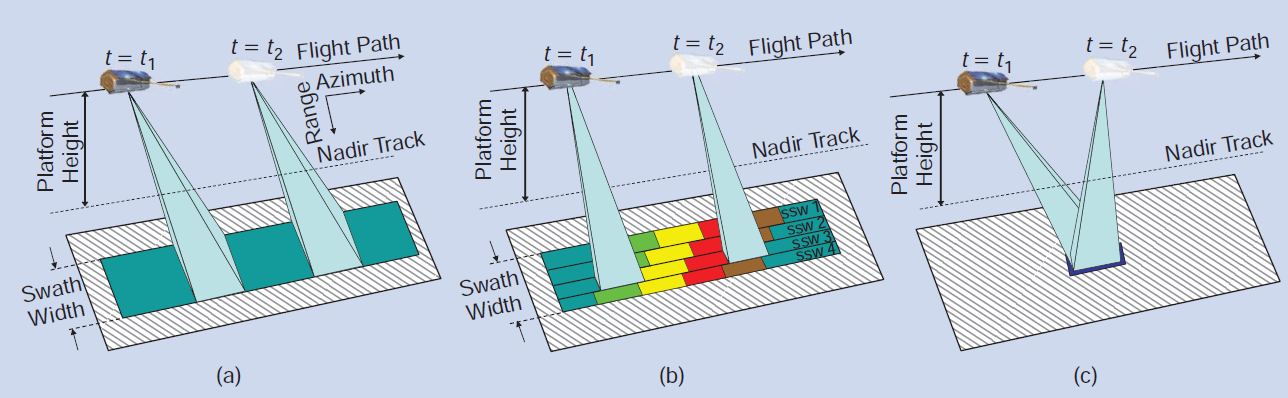
\includegraphics[width=0.5\textwidth]{Bilder/SAR_Modi.png}
    \caption{Aufnahmeverfahren SAR Systemen \cite{tutorial_on_sar}}
    \label{fig:sar_prinzip}
\end{figure}

Im Gegensatz zu optischen Aufnahmeverfahren liefern die Rohdaten 
einer Befliegung mit Radarsensoren noch keine Bilddaten. Um Bilder zu erzeugen, bedarf es zunächst einer komplexen Verarbeitung der aus Amplitude und Phase bestehenden. 
Signale. Dabei werden die Daten entlang des Azimuts und der Blickrichtung gefiltert. In der Regel repräsentieren die Pixelwerte eines aus Radardaten abgeleiteten Bildes 
der Reflektivität der korrespondierenden Fläche. Mittels Geocodierung kann das so entstandene Bild verortet werden. Zusätzlich können diverse Kalibrierungen vorgenommen 
werden. Dazu gehören Verfahren welche Rauscheffekte minimieren, die geometrischen Eigenschaften verbessern oder die Interpretation der Bilder erleichtern \cite{tutorial_on_sar}. 

\subsection{Copernicus Programm}
\subsubsection{Ziele}
Das Copernicus Programm ging aus dem Global Monitoring for Environmental Security Programm (GMES) Programm hervor welches 1998 mit dem Ziel initiiert wurde um Europa 
zu ermöglichen eine führende Rolle bei der Lösung von weltweiten Problemen im Kontext Umwelt und Klima zu verschaffen. Teil dieser Bestrebungen ist der Aufbau eines 
leistungsfähigen Programms zur Erdbeobachtung. 2012 wurde das GMES-Programm zum Copernicus Programm umbenannt \cite{history_of_copernicus}.
Erklärte Ziele des Copernicus Programmes ist das Überwachen der Erde um den Schutz der Umwelt sowie Bemühungen von Katastrophen- und Zivilschutzbehörden zu 
unterstützen. Gleichzeitig soll die Wirtschaft im Bereich Raumfahrt und der damit verbundenen Services unterstützt und Chancen für neue Unternehmungen geschaffen
werden \cite{copernicus_regulation}.

\subsubsection{Aufbau}
Das Copernicus Programm besteht aus Weltraum, In-Situ- und Service-Komponente. 
Zur Weltraum-Komponente gehören die verschiedenen Satellitenmissionen sowie Bodenstationen welche für den Betrieb sowie die Steuerung und Kalibrierung  der 
Satelliten verantwortlich sind \cite{copernicus_regulation}. Sentinel-1 Satelliten sind mit bildgebenden Radarsystemen ausgerüstet und beobachten wetter- und 
tageszeitunabhängig Land-, Wasser- und Eismassen um unter andrem das Krisenmanagement zu unterstützen. Satelliten der Sentinel-2 Mission führen hochauflösende, 
multispektrale Kameras mit und liefern weltweit optische Fernerkundungsdaten. Altimetrische und radiometrische Daten von Land- und Wasserflächen werden von der 
Sentinel-3 Satellitenmission gesammelt während spektrometrische Daten zur Überwachung der Luftqualität von Sentinel-4 und 5 Satelliten erfasst werden. 
Ozeanografische Daten sollen von den Setinel-6 Satelliten geliefert \cite{sentinel_overview}. \\

Die In-Situ-Komponente sammelt Daten von see-, luft- und landbasierten Sensoren sowie geografische und geodätische Referenzdaten. Die harmonisierten Daten 
werden verwendet um die Daten der Weltraum-Komponente zu verifizieren oder zu korrigieren. Gleichzeitig können räumliche oder thematische Lücken in der 
Datenabdeckung gefüllt werden \cite{copernicus_regulation}\cite{what_is_copernicus}. \\

Zur Service-Komponente gehören unterschiedliche Dienste welche jeweils auf Themengebiet abgestimmt sind und Daten in hoher Qualität bereitstellen.
Der Copernicus Atmosphere Monitoring Service (CAMS) soll Informationen zur Luftqualität und der chemischen Zusammensetzung der Atmosphäre liefern. 
Daten bezüglich des Zustands und der Dynamik der Meere und deren Ökosysteme lassen sich über den Copernicus Marine Environment Monitoring Service (CMEMS) beziehen. 
Informationen zur Flächennutzung und und Bodenbedeckung werden vom Copernicus Land Monitoring Service (CLMS) bereitgestellt. 
Um eine nachhaltige Klimapolitik planen und umsetzen zu können stellt der Copernicus Climate Change Service (C3S) aktuelle sowie historische Klimadaten bereit.  
Um den Zivilschutzbehörden schnelle Reaktionen auf Umweltkatastrophen zu ermöglichen stellt der  Emergency Management Service (EMS) entsprechende Fernerkundungsdaten 
breit. Ähnliche Daten können von europäischen Zoll- und Grenzschutzbehörden über den Copernicus Security Service bezogen werden
\cite{copernicus_regulation}\cite{what_is_copernicus}.

\subsubsection{Sentinel 1}
Die Sentinel-1 Satellitenmission liefert wetter- und tageszeitunabhängige Radardaten der Erdoberfläche. Die Mission besthet aus zwei Staelliten, Sentinel-1 A und B,
sowie einer Bodenkomponente welche für Steuerung und Kalibrierung und Datenverarbeitung verantwortlich ist. Die Satelliten tragen als Hauptinstrument ein 
bildgebendes Radar mit synthetischer Apertur welches im C-Frequenzband arbeitet. Es stehen zwei Polarisationsmodi, Single (HH, VV) oder Dual (HH+HV, VV+VH),
zur Verfügung \cite{sentinel_1_definition}. 
Die Erfassung von Daten kann in vier Aufnahmemodi erfolgen welche sich in Auflösung, Streifenbreite und Anwendungsszenario unterscheiden. 
Der Standardmodus ist der Stripmap Modus (SM) bei dem Aufnahmestreifen mit einer kontinuierlichen Folge von Signalen abgetastet wird \cite{sentinel_1_definition}.
Die Aufnahmemodi Interferometric Wide Swath Mode (IW) und Extra-Wide Swath Mode (EW) arbeiten im TOPSAR Verfahren mit drei beziehungsweise
fünf Sub-Aufnahmestreifen um ein größeres Gebiet aber in geringerer Auflösung aufnehmen zu können. TOPSAR ist eine Abwandlung des ScanSAR Verfahrens bei 
dem die Antenne zusätzlich in Azimutrichtung vor und zurück bewegt wird um die radiometrische Qualität der resultierenden Bilder zu verbessern. 
Wenn der Wave Modus (WV) zu Einsatz kommt werden kleine, Vignetten genannte, Szenen im Stripmap Verfahren aufgenommen. Sie werden in regelmäßigen Abständen und
wechselnden Depressionwinkeln aufgenommen \cite{tutorial_on_sar}\cite{sentinel_1_definition}.   

\begin{figure}[H]
    \centering
    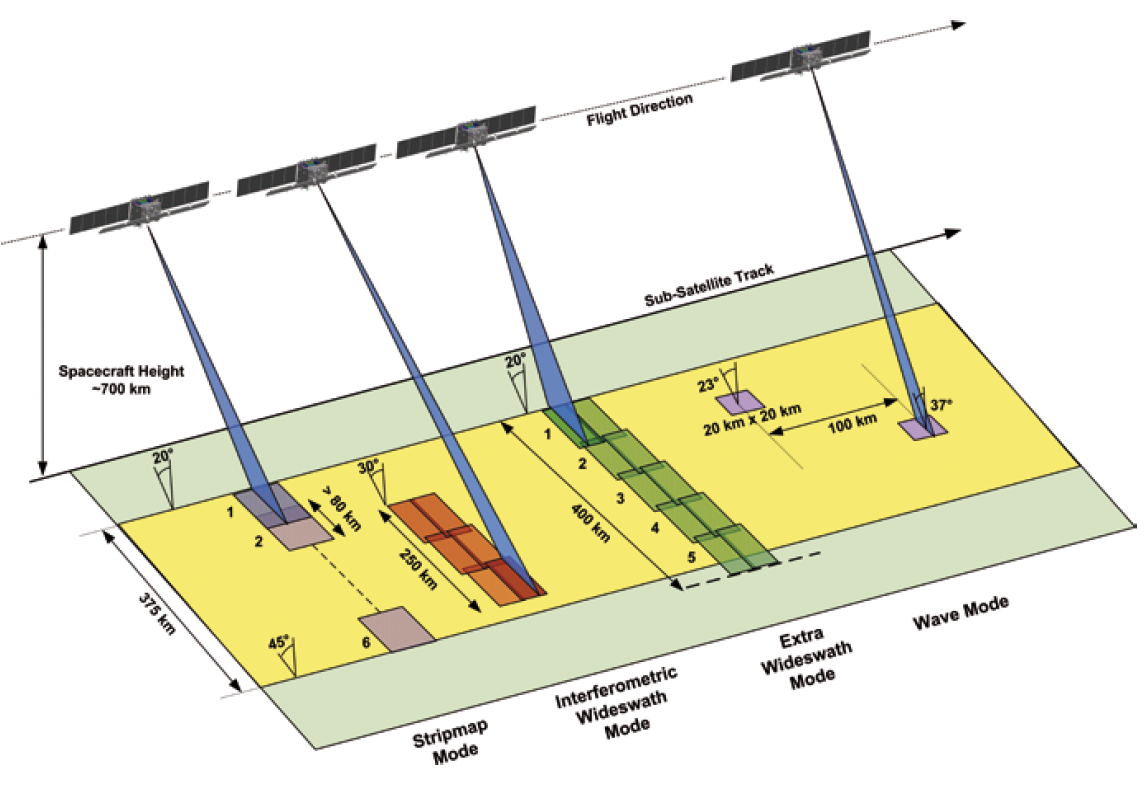
\includegraphics[width=0.5\textwidth]{Bilder/Aquisition_Modes.png}
    \caption{Aufnahmemodi der Sentinel-1 Mission \cite{sentinel_1_overview}}
    \label{fig:aquisition_modes}
\end{figure}

\begin{center}
\begin{table}[H]
    \caption{Eigenschaften der Aufnahmemodi der Sentinel-1 Mission \cite{sentinel_1_overview}}
    \centering
    \begin{tabular}{|c|c|c|c|c|} 
        Modus & IW & WV & SM & EW \\ 
        \hline
        Polarisation & Dual & Single & Dual & Dual \\ 
        Azimut-Auflösung (m) & 20 & 5 & 5 & 40 \\
        Rage-Auflösung (m) & 5 & 5 & 5 & 20 \\
        Streifenbreite (km) & 250 & 20x20 & 80 & 410\\
    \end{tabular}
    \label{table:1}
\end{table}
\end{center}

Beide Satelliten befinden sich auf einem polnahen, sonnensychronen Orbit. Ein Zyklus dauert 12 Tage in denen die Erde 175 umrundet wird. Da er sich um ein Satellitenpaar
handelt welches als Tandem die Erde umrundet wird ein Punkte alle sechs Tage von einem der Satelliten überflogen. Das System kann eine zuverlässige globale und systematische
Abdeckung liefern. Dabei können im IW Modus alle relevanten Land-, Wasser- und Eismassen alle zwölf Tage vollständig von einem Satelliten erfasst werden. 
In Krisensituationen können nach Bedarf innerhalb von zweieinhalb und fünf Tagen Daten erfasst werden \cite{sentinel_1_overview}. 

Nach dem Erfassen der Daten und dem Übersenden an eine Bodenstation werden diverse Vorverarbeitungsschritte vorgenommen in die sowohl interne also auch externe
Parameter einfließen. Daraus ergeben sich diverse Produkte welche sich durch Aufnahmemodus (IW, SM, EW und WV), Level-1 Produkt-Typ (SLC, GRD) sowie ihre 
Auflösung (Full-, High-, und Medium-Resolution) unterscheiden. Single Look Complex (SLC) Produkte sind im wesentlichen Kalibrierte Rohdaten in denen Amplitude und Phase nicht
zur Reflektivität kombiniert wurden und die geometrische Auflösung sich in Azimut- und Blickrichtung unterscheidet. Ground Rage Detected (GRD) Produkte bilden hingegen die 
Reflektivität ab und haben eine annähern quadratische geometrische Auflösung. Die Reflektivität wird in der logarithmischen Maßeinheit Decibel (dB). Die Korrektur der Auflösung 
in Blickrichtung erfolgt dabei erfolgt dabei durch Projektion auf einen Ellipsoiden. \cite{sentinel_1_definition}. Aus den Level-1 Produkten können die Level-2 Produkte 
OSW, OWI und RVL abgeleitet werden.

\subsubsection{Datenzugang}
\subsection{Überschwemmungsmonitoring}
\subsection{Schnittstellen}
\subsection{OGC und OGC Standards}
\subsection{OGC API - Processes - Part 1: Core}
\subsubsection{Ziele}
\subsubsection{Aufbau}
\subsection{Evaluationskriterien}

